\section{Conclusion and Future Work}
We present a compact representation of PRT for \textbf{free form} deformable objects, in form of a non-linear model, namely a deep convolutional neural network, with enormous memory saving potential.
 The model is able to extract the features of the dataset relevant to self-shadowing and thus generate good approximations for a wide spectrum of deformations, with resulting appearances that are visually indistinguishable from the ground truth.  
\\
Moreover, our method shows much higher generalization properties than previous approaches allowing deformations from much larger and less constrained deformation spaces.
\\
\\
Although we showed DeepPRT can be much more compact than traditional PRT, our network is far from being optimal. Exploiting network compression and acceleration methods could highly benefit DeepPRT \cite{Survey_NN_Compression}, \cite{Deep_Compression}.
Moreover, other network topologies and/or cost functions could be explored in order to achieve  better approximations, for instance, as proposed in \cite{Deformable_UNet} to account for individual object deformations the use of deformable convolutions \cite{DeformableCNN} could be investigated.
\\
The particular choice of our basis functions (Spherical Harmonics), currently restricts our method to low-frequency lightings. However, an extension to all-frequencies is possible by fitting the model to an alternative representation of the transfer function $T$, such as non-linear Wavelets \cite{AllFrequencyPRT}.
\\
The most significant limitations of our method reside within the choice of our parametrisation (harmonic map) and the natural flaws of the geometry images surface representation.  Currently, DeepPRT only performs well for modest curvature variations and is restricted to surfaces with one boundary (topological disks); however, using the geometric-stretch parametrisation instead and further using the extension proposed by \cite{Spherical_Parametrization}, the shape representation would be more robust and applicable to more general surfaces. 
%%%%%%%%%%%%%%%%%%%%%%%%%%%%% 
%\textit{\begin{figure*}
%  \centering
%    \includegraphics[width=0.7\paperwidth]{Figures/DPRT_quality_SSIM.pdf}
%     \caption{Prediction Quality:
%     a : ground truth appearance. b: predicted appearance. c: SSIM. d: L1-Error between ground truth and predicted transfer coefficients }
%     \label{Fig: DPRT_Quality}
%\end{figure*}}
\begin{figure}[H]
  \centering
    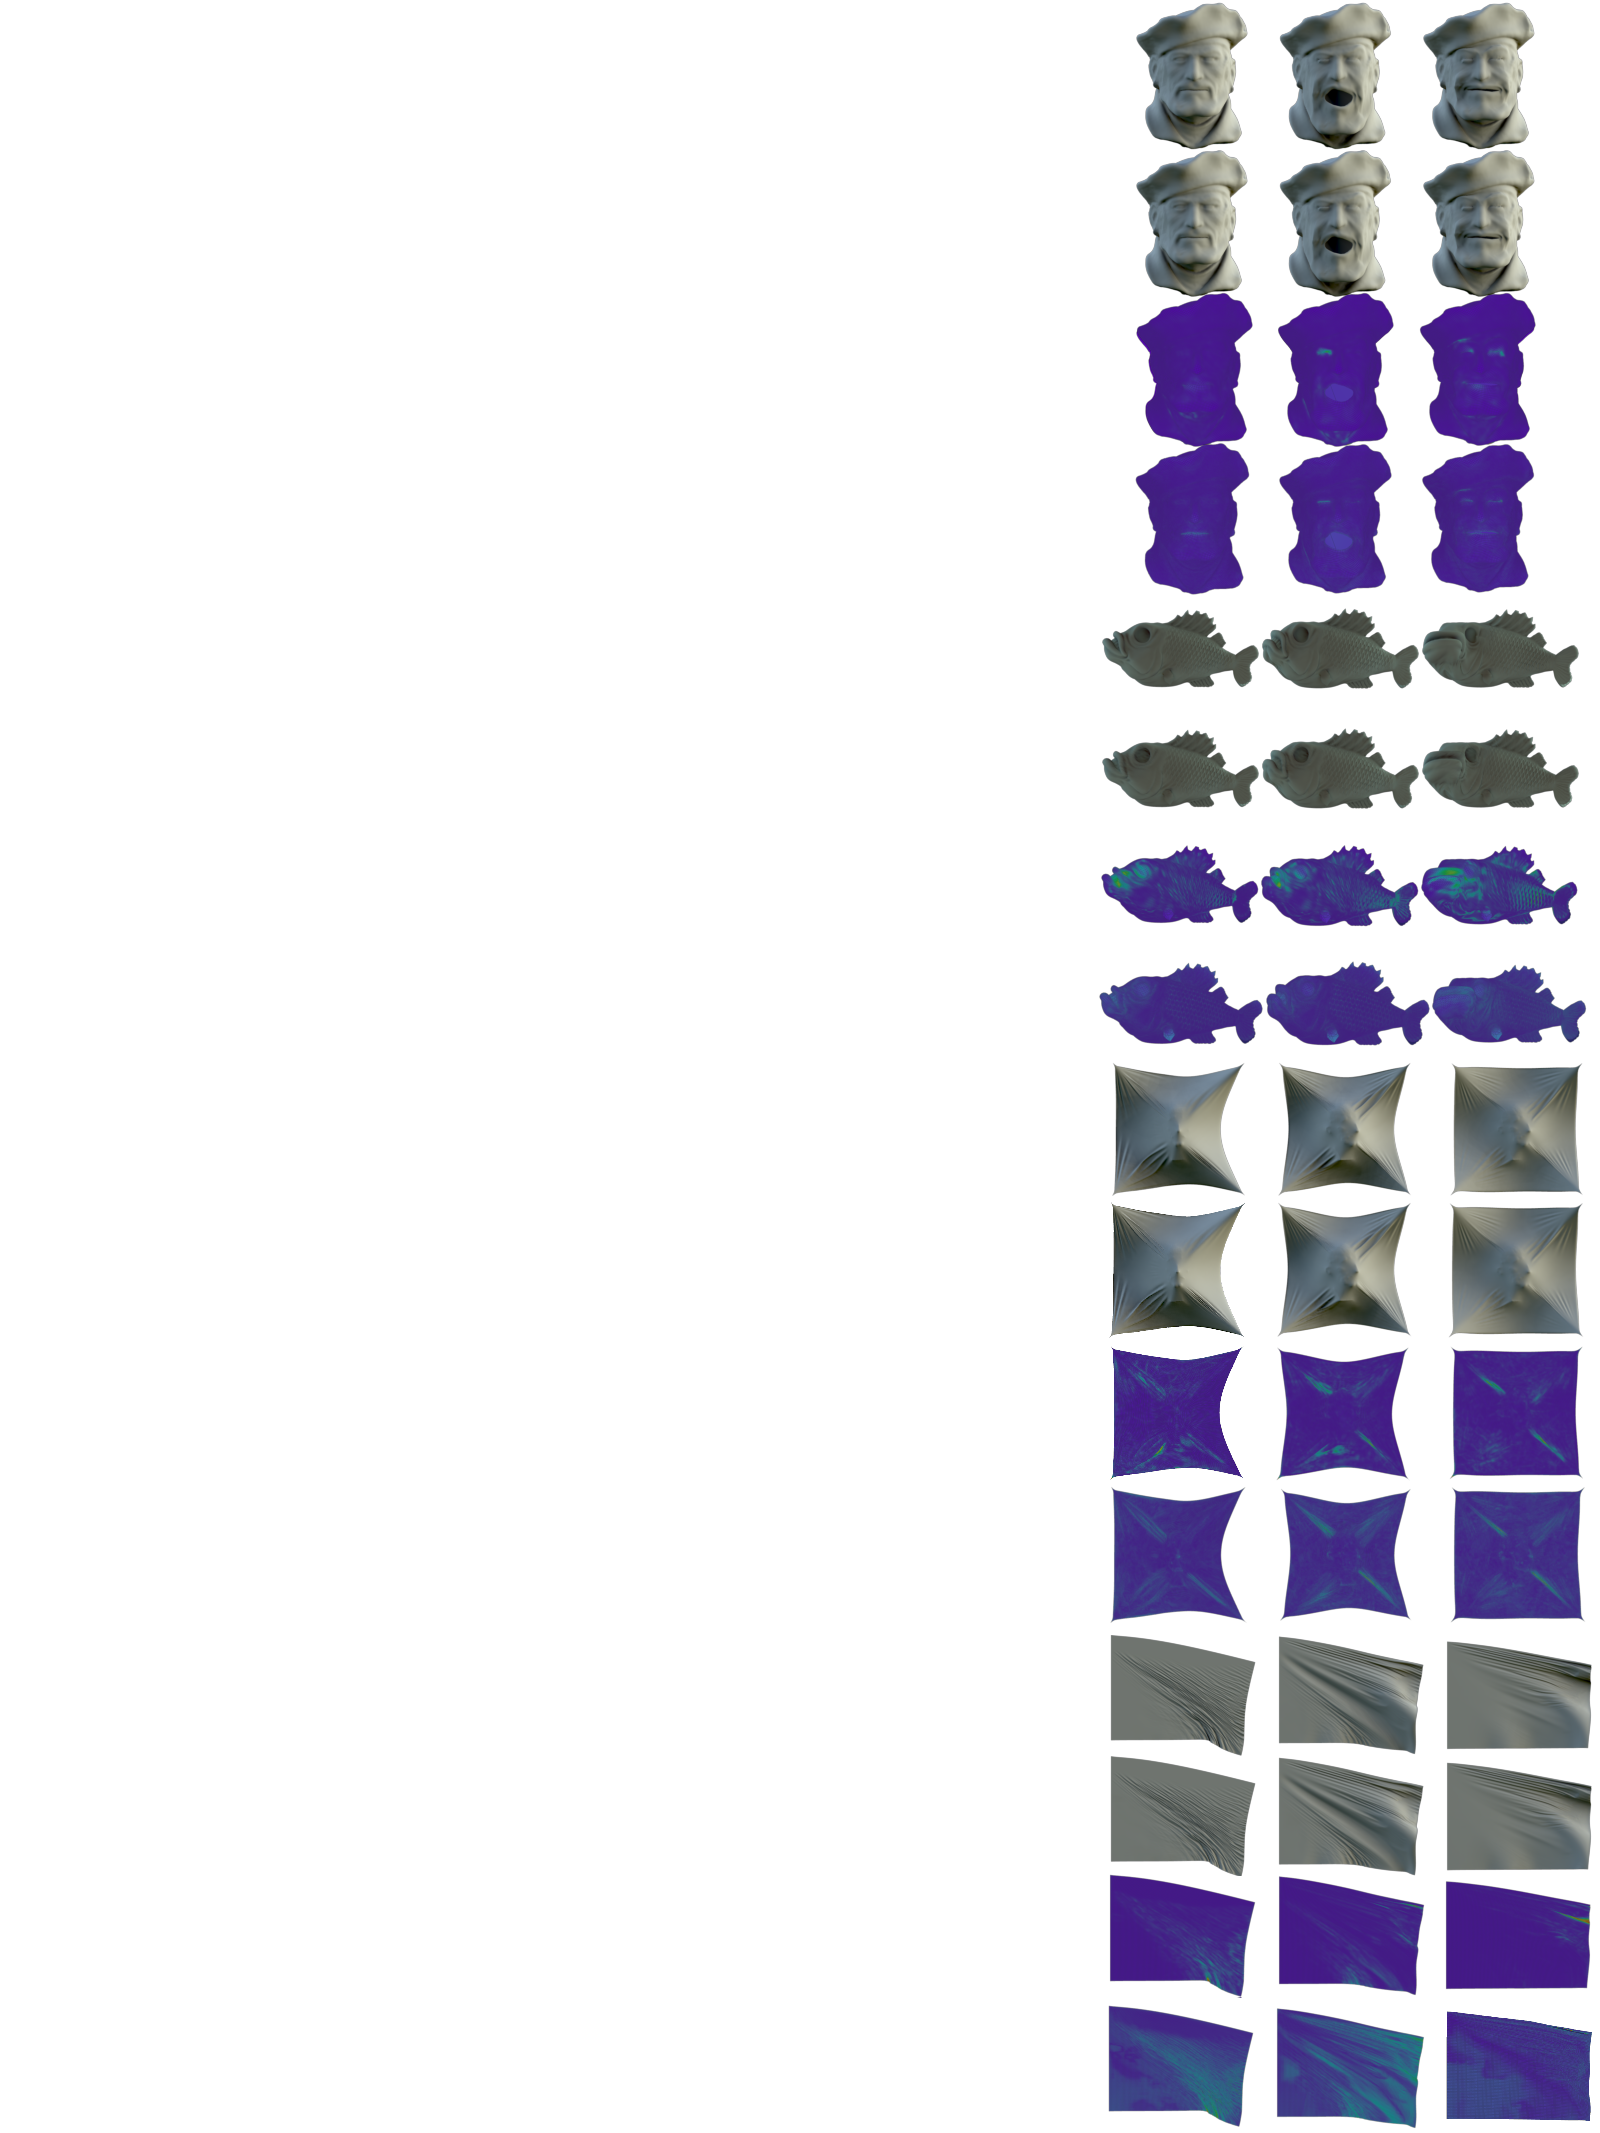
\includegraphics[height=\textheight]{Figures/DPRT_quality_SSIM_vert.pdf}
     \caption{Prediction Quality:
     a : ground truth appearance. b: predicted appearance. c: SSIM. d: L1-Error between ground truth and predicted transfer coefficients }
     \label{Fig: DPRT_Quality}
\end{figure}